\documentclass{article}

\def\sectionnumber{7}
\def\sectiontitle{Joint Distributions, Covariance and Correlation, Multinomial}

\usepackage{common}

% Set this false to hide, true to show
\setboolean{showanswers}{false}

\begin{document} 

\header

\section{Joint Distributions}

\begin{description}

\item[Joint PMF] $p_{X, Y}(x, y) = P(X=x, Y=y)$

\item[Marginal PMF] $p_{X}(x) = \sum_y P(X=x, Y=y)$.

\item[Conditional PMF] $P(X=x|Y=y)$

\item[Continuous analogues] Replace all the PMFs with PDFs, and replace all the sums with integrals.


\end{description}

% 3. (BH 7.9) Let $X$ and $Y$ be i.i.d.~$\Geom(p)$, and $N = X+Y$. 

% (a) Find the joint PMF of $X$, $Y$, and $N$. 

% \hide{We want to compute $P(X=x,Y=y,N=n)$ for all nonnegative integers $x$, $y$, $n$. If $n \neq x+y$, then this probability is clearly zero, so the PMF is only nonzero when $n = x+y$. But then $N=n$ is redundant information, so $P(X=x,Y=y,N=n) = P(X=x,Y=y) = P(X=x)P(Y=y) = p^2(1-p)^{x+y} = \boxed{p^2(1-p)^{n}}$ where we used independence for the second equality.}

% (b) Find the joint PMF of $X$ and $N$. 

% \hide{$P(X=x,N=n) = P(X=x,Y=n-x) = P(X=x)P(Y=n-x) = \boxed{p^2(1-p)^n}$ for all nonnegative integers $x$ and $n$ with $n \geq x$. Note that this is the same as above...since you only need any two of $X$, $Y$, and $N$ to get all the information in the problem.}

% (c) Find the conditional PMF of $X$ given $N=n$, and give a simple description of what the result says. 

% \hide{$P(X=x|N=n) = \frac{P(X=x,N=n)}{P(N=n)}$ by the definition of conditional probability. $N \sim \NBin(2, p)$, so by the PMF of the negative binomial we have $P(N=n) = (n+1)p^2(1-p)^n$. Plugging our result from part (b) for the numerator gives $\boxed{\frac{1}{n+1}}$ for all $x \in \{0,1,\dots,n\}$. This means that it is equally likely for $X$ to be any of these values.}

({\bf Random sphere}) Consider choosing a random point in the unit sphere:
$$\{(x, y, z) : x^2 + y^2 + z^2 \leq 1\}.$$ We can represent this ``random choice" as three random variables, each representing a coordinate: $(X, Y, Z)$.

(a) Find the joint PDF of $X, Y, Z$.

\hide{Since the total volume of the sphere is $\frac{4\pi}{3}$, we must have the PDF as $f_{X,Y,Z}(x, y, z) = \frac{3}{4\pi}$ due to the uniform nature of the distribution.}

(b) Find the marginal distribution of $X$.

\hide{To find the marginal distribution, we must integrate out the other random variables $Y, Z$,
resulting in:

$$\int_{-\sqrt{1 - x^2}}^{\sqrt{1 - x^2}} \int_{-\sqrt{1 - x^2 - z^2}}^{\sqrt{1 - x^2 - z^2}} \frac{3}{4\pi} dydz$$
which is best left as an integral as it is difficult to compute analytically.
}

(c) Find the probability that $(X, Y, Z)$ lies in a smaller sphere of radius 0.5.

\hide{To solve this problem, we note that because the density is uniform, the question of finding
the probability of locating a point in a given region is simply the volume of that region divided by the
total volume, which is $\frac{4\pi}{3}$. Thus, we have:
$$P((X, Y, Z) \in B_{0.5}) = \frac{\frac{4\pi(0.5)^3}{3}}{\frac{4\pi}{3}} = \frac{1}{8}.$$
}

({\bf Uniforms}) Let $U_1$, $U_2$, $U_3$ be i.i.d.~Unif(0,1), and let $L=\min(U_1,U_2,U_3)$, $M=\max(U_1,U_2,U_3)$.

(a) Find the marginal CDF and marginal PDF of $M$, and the joint CDF and joint PDF of $L$, $M$.

Hint: for the latter, start by considering $P(L\geq l,M\leq m)$.

\hide{
The event $M \leq m$ is the same as the event that all 3 of the $U_j$ are at most $m$, so the CDF of $M$ is $F_M(m) = m^3$ and the PDF is $f_M(m)=3m^2$, for $0 \leq m \leq 1$.

The event $L \geq l$, $M \leq m$ is the same as the event that all 3 of the $U_j$ are
between $l$ and $m$ (inclusive), so
$P(L \geq l, M \leq m)=(m-l)^3$
for $m\geq l$ with $m, l \in [0, 1]$. By the axioms of probability, we have
$P(M \leq m) = P(L \leq l,M \leq m) + P(L > l,M \leq m)$.

So the joint CDF is
$$P(L \leq l,M \leq m) = m^3-(m-l)^3,$$
for $m\geq l$ with $m, l \in [0, 1]$. The joint PDF is obtained by differentiating this
with respect to $l$ and then with respect to $m$ (or vice versa):
$$f(l, m) = 6(m-l),$$
for $m\geq l$ with $m, l \in [0, 1]$. As a check, note that getting the marginal PDF of
$M$ by finding $\int^m_0 f(l, m)dl$ does recover the PDF of $M$ (the limits of integration are from 0 to $m$ since the min can’t be more than the max).
}

(b) Find the conditional PDF of $M$ given $L$.

\hide{
The marginal PDF of L is $f_L(l) = 3(1-l)^2$ for $0 \leq l \leq 1$ since $$P(L>l) = P(U_1 > l, U_2 > l, U_3 > l) = (1-l)^3$$ (alternatively, use the PDF of $M$ together
with the symmetry that $1-U_j$ has the same distribution as $U_j$ , or integrate
out $m$ in the joint PDF of $L, M$). So the conditional PDF of $M$ given $L$ is
$$f_{M|L}(m|l) = \frac{f(l, m)}{f_L(l)} = \frac{2(m-l)}{(1-l)^2}$$
for all $m, l \in [0, 1]$ with $m\geq l$.
}

\section{Covariance and Correlation}

\begin{description}

\item[Covariance] $\cov(X, Y) = E[(X - EX)(Y - EY)] = E(XY) - E(X)E(Y)$. The covariance of independent r.v.s is 0, but if two r.v.s have covariance 0, they aren't necessarily independent.

\item[Key properties of covariance] These almost always come in handy when covariances pop up.

    \begin{enumerate}
        \item $\cov(X, X) = \var(X)$
        
        \item $\cov(X, Y) = \cov(Y, X)$
        
        \item $\cov(X, c) = \cov(c, X) = 0$ for any constant $c$
        
        \item $\cov(aX, Y) = a\cov(X, Y)$ for any constant $a$
        
        \item $\cov(X + Z, Y) = \cov(X, Y) + \cov(Z, Y)$ -- covariance is distributive (very similar to multiplication)
        
        \item $\var(X_1 + \dots + X_n) = \var(X_1) + \dots + \var(X_n) + 2\sum_{i < j} \cov(X_i, X_j)$
    \end{enumerate}

\item[Correlation] $\corr(X, Y) = \frac{\cov(X, Y)}{\SD(X)\SD(Y)}$. Correlation $\rho$ always satisfies $-1 \leq \rho \leq 1$. Note that independent variables always have correlation zero, but the converse is not generally true (unless you're working with a Multivariate Normal)

\end{description}

({\bf Stock portfolios}) Mark is thinking about constructing a portfolio of two stocks: A and B. Suppose the annual percentage return $R_A$ of stock A is distributed as $\N(\mu=10, \sigma^2=25)$, while those of stock B (call it $R_B$) are distributed as $\N(\mu=5, \sigma^2=9)$. Suppose $\corr(R_A,R_B) = -0.5$. For every share of stock $A$ in Mark's portfolio, how many shares of stock $B$ should he buy to minimize the variance of his portfolio's returns?

\hide{Say Mark buys $b$ shares of stock $B$ per share of stock $A$. Then Mark's portfolio return per share of stock $A$ is given by $R \equiv R_A + bR_B$. We compute
\begin{align*}
    \var(R) & = \var(R_A+bR_B) \\
    & = \cov(R_A+bR_B,R_A+bR_B) \\
    & = \var(R_A) + 2b\cov(R_A,R_B) + b^2\var(R_B) \\
    & = 25 - 15b + 9b^2
\end{align*}
where we've computed $\cov(R_A,R_B) = \corr(R_A,R_B) \cdot \SD(R_A)\SD(R_B) = -7.5$. This expression is minimized when $b = \frac{15}{18} = \boxed{\frac{5}{6}}$.} 

({\bf Secret Santa}) For Christmas, $n$ people are doing a Secret Santa, where each person puts his or her name on a piece of paper in a hat and randomly picks a name from the hat without replacement. In this game, there is a possibility that people can select their own names and have to buy themselves a gift. :( 

\begin{figure}[!ht]
\begin{center}
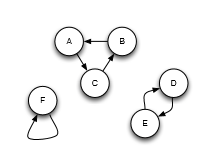
\includegraphics[width = 0.3\textwidth]{cycle.PNG}
\end{center}
\end{figure}

(a) What is the expected number of cycles that form? (Three examples of cycles are shown.)

\hide{First we define the random variable of interest as $X$, where $X$ is the number of cycles that form. Next, we break up $X$ into its indicator random variables. We would like to count the number of cycles that happen on a person by person basis, so we split up $X$ into indicators that the $i$th person in Secret Santa completes a cycle after drawing a name from the hat. We have 
\[X = I_1 + I_2 + ... + I_n\]
We apply linearity of expected value and the fundamental bridge to express the expected value of $X$ in terms of the probabilities of each of the $n$ events:
\[E(X) = P(I_1=1) + P(I_2=1) + ... + P(I_n=1)\]
We note that $P(I_1 = 1/n)$: for the first person to choose, the only way that person will form a cycle is if that person chooses himself/herself. Continuing, $P(I_2 = 1/(n-1))$, as there are $n-1$ remaining choices in the hat, and only one of the draws will lead to a completed cycle (it could be the person himself/herself, or it could be the person who drew that person from the hat). The pattern continues until $P(I_n = 1)$ -- the last person who draws will always complete a cycle -- so
\[E(X) = \sum_{k=1}^n \frac{1}{k}\]
}


(b) What is the variance of the number of cycles that are formed? \\

\hide{Continuing from the previous question,
\[\var(X) = \var(I_1 + I_2 + ... + I_n) \]
and we can apply the properties of covariance as follows:
\begin{align*}
    \var(X) &= \cov(I_1 + I_2 + ... + I_n, I_1 + I_2 + ... + I_n) \\
    &= \cov(I_1, I_1) + \cov(I_2, I_2) + ... + \cov(I_n, I_n) + \sum_{i \neq j} \cov(I_i, I_j) \\
    &= \sum_{i=1}^n \var(I_i) + 2\sum_{i < j} \cov(I_i, I_j)
\end{align*}
Now note that $I_i$ and $I_j$ are independent, since knowing that $i$ forms a cycle does not affect the probability that $j$ forms a cycle; $E(I_i) = P(I_i = 1) = 1/(n-i+1)$ regardless of how many cycles have already been formed. The covariances therefore drop out, and we obtain
\begin{align*}
    \var(X) &= \sum_{i=1}^n \var(I_i) \\
    &= \sum_{i=1}^n \left( E(I_i^2) - [E(I_i)]^2 \right)\\
    &= \sum_{i=1}^n \left( E(I_i) - [E(I_i)]^2 \right) \\ 
    &= \sum_{i=1}^n \left( \frac{1}{i}\ -\left(\frac{1}{i}\right)^2 \right)\\ 
\end{align*}
}

\section{Multinomial}

\begin{description}

\item[Story] Each of $n$ objects is placed randomly and independently into $k$ categories. The probability of being placed into category $i$ is $p_i$. Let $\mathbf{p} = (p_1, p_2, \dots, p_k)$. Then the distribution of the number of objects in each category is $\Mult_k(n, \mathbf{p})$. This is a generalized version of the Binomial (the $j$th element of a $\Mult_k(n, \mathbf{p})$ random vector is distributed as a $\Bin(n, p_j)$).

\item[Joint PMF] $$P(X_1 = n_1, X_2 = n_2, \dots, X_k = n_k) = \frac{n!}{n_1!n_2!\cdots n_k!}p_1^{n_1}p_2^{n_2}\cdots p_k^{n_k}$$ You don't really have to remember this, but know that this is the generalization of the Binomial PMF.

\item[Lumping] If you lump more than one of the $k$ categories together, the result is still Multinomial. For example, lumping categories 1 and 2 together results in a Multinomial with new probability $p_1 + p_2$.

\end{description}

({\bf Higgs Boson}) On July 4, 2012, the state of humanity's understanding of the universe took a large step forward with the discovery of the Higgs boson. Put simply, the way to discover the Higgs boson is to collide particles at high enough energies so that the boson is produced. Unfortunately, it decays extremely quickly into a bunch of elementary particles. For simplicity, let's suppose that a Higgs boson decays into one of three possible pairs: 1) fermion pair; 2) W boson pair; 3) Z boson pair. The events occur with probabilities $p$, $q$, and $1-p-q$, respectively. 

(a) What is the PMF of $F, W, Z$, signifying the number of times each of the decay events occur, given that we produce $n$ Higgs bosons?

\hide{$F, W, Z \sim \Mult_3(n, (p, q, 1 - p - q))$}

(b) What is the distribution of the number of fermion pair decays?

\hide{By lumping, we have: $F \sim \Bin(n, p)$.}


\end{document}

